\documentclass[11pt,a4paper]{article}

% ════════════════════════════════════════════════════════════
% Packages
% ════════════════════════════════════════════════════════════
\usepackage[margin=2.5cm]{geometry}
\usepackage{amsmath,amssymb}
\usepackage{booktabs,array,multirow,colortbl,makecell}
\usepackage{tikz}
\usetikzlibrary{arrows.meta,positioning,shapes,automata,calc,fit}
\usepackage{listings}
\usepackage[most]{tcolorbox}
\usepackage[ruled,vlined]{algorithm2e}
\usepackage{qrcode}
\usepackage[colorlinks=true,linkcolor=blue!60!black,urlcolor=blue!60!black,citecolor=blue!60!black]{hyperref}
\usepackage{titlesec}
\usepackage{enumitem}
\usepackage{xcolor}
\usepackage{caption}
\usepackage{subcaption}
\usepackage{fancyhdr}
\usepackage{lastpage}

% ════════════════════════════════════════════════════════════
% Colors
% ════════════════════════════════════════════════════════════
\definecolor{nodeblue}{HTML}{C5D9F1}
\definecolor{nodegreen}{HTML}{C3E6CB}
\definecolor{nodeorange}{HTML}{FFD8B2}
\definecolor{nodeyellow}{HTML}{FFF2CC}
\definecolor{nodepurple}{HTML}{E2D5F0}
\definecolor{nodered}{HTML}{F4CCCC}
\definecolor{mayblue}{HTML}{4472C4}
\definecolor{codebg}{HTML}{F5F5F5}

% ════════════════════════════════════════════════════════════
% Callout Boxes
% ════════════════════════════════════════════════════════════
\newtcolorbox{infobox}[1][Info]{
  colback=blue!5,
  colframe=blue!60!black,
  title=#1,
  fonttitle=\bfseries,
  boxrule=1pt,
  arc=3pt
}
\newtcolorbox{warningbox}[1][Warning]{
  colback=orange!5,
  colframe=orange!70!black,
  title=#1,
  fonttitle=\bfseries,
  boxrule=1pt,
  arc=3pt
}
\newtcolorbox{dangerbox}[1][Danger]{
  colback=red!5,
  colframe=red!60!black,
  title=#1,
  fonttitle=\bfseries,
  boxrule=1pt,
  arc=3pt
}

% ════════════════════════════════════════════════════════════
% Listings Style
% ════════════════════════════════════════════════════════════
\lstset{
  basicstyle=\small\ttfamily,
  backgroundcolor=\color{codebg},
  frame=single,
  framerule=0.4pt,
  rulecolor=\color{gray!40},
  breaklines=true,
  numbers=left,
  numberstyle=\tiny\color{gray},
  keywordstyle=\color{blue!70!black}\bfseries,
  commentstyle=\color{green!50!black}\itshape,
  stringstyle=\color{red!60!black},
  showstringspaces=false,
  tabsize=4,
  xleftmargin=2em,
  framexleftmargin=1.5em,
}
\lstdefinelanguage{bash}{
  morekeywords={sudo,ls,pip,install},
  morecomment=[l]{\#},
  morestring=[b]",
}

% ════════════════════════════════════════════════════════════
% TODO checkbox
% ════════════════════════════════════════════════════════════
\newcommand{\todo}[1]{\item[$\square$] #1}

% ════════════════════════════════════════════════════════════
% Page Style
% ════════════════════════════════════════════════════════════
\pagestyle{fancy}
\fancyhf{}
\fancyhead[L]{\small Low-Cost UMI Report}
\fancyhead[R]{\small\thepage/\pageref{LastPage}}
\renewcommand{\headrulewidth}{0.4pt}

% ════════════════════════════════════════════════════════════
% Title
% ════════════════════════════════════════════════════════════
\title{\textbf{Low-Cost UMI Report}\\[0.3em]
\large A Wireless Bimanual Data Collection System for Imitation Learning\\
with NRF24L01+ Time Synchronization}
\author{}
\date{}

\begin{document}
\maketitle
\thispagestyle{fancy}
\tableofcontents
\newpage

% ════════════════════════════════════════════════════════════
% 1. Introduction
% ════════════════════════════════════════════════════════════
\section{Introduction}

This report presents a \textbf{low-cost wireless bimanual data collection system} designed for imitation learning on the SO-101 robot arm. Each gripper unit captures 6DoF pose via T265 VIO, fisheye and RGB observation images, and gripper aperture from the STS3215 encoder---all logged onboard a Raspberry Pi 4B. Two grippers are synchronized via \textbf{NRF24L01+ Enhanced ShockBurst} (ESB) with hardware ACK payload, achieving ${\sim}0.8$\,ms round-trip time and ${\sim}0.2$\,ms synchronization error through symmetric time synchronization.

\begin{table}[htbp]
\centering
\caption{System comparison. Ours uses NRF24L01+ radio and dual cameras while remaining fully wireless.}
\begin{tabular}{l c c c}
\toprule
\textbf{Feature} & \textbf{UMI} & \textbf{FastUMI} & \textbf{Ours} \\
\midrule
Observation & GoPro RGB & GoPro RGB & T265 fisheye + USB RGB \\
Pose tracking & ORB-SLAM3 & T265 VIO & T265 VIO \\
Gripper width & Vision & ArUco & STS3215 encoder \\
Cameras / gripper & 1 & 2 & \textbf{2} \\
Synchronization & --- & --- & \textbf{NRF24L01+ ESB} \\
Compute & PC offline & Laptop + ROS & \textbf{RPi onboard} \\
Tethered & No & USB cable & \textbf{None} \\
\bottomrule
\end{tabular}
\end{table}


% ════════════════════════════════════════════════════════════
% 2. System Architecture
% ════════════════════════════════════════════════════════════
\section{System Architecture}

% ─────────────────────────────────────────────────
% 2.1 Hardware Architecture
% ─────────────────────────────────────────────────
\subsection{Hardware Architecture}

Each gripper unit contains 9 components: T265 camera, USB RGB camera, RPi 4B, NRF24L01+ radio, STS3215 servo, SD card, button/LED, LiPo battery with UBEC.

\begin{figure}[htbp]
\centering
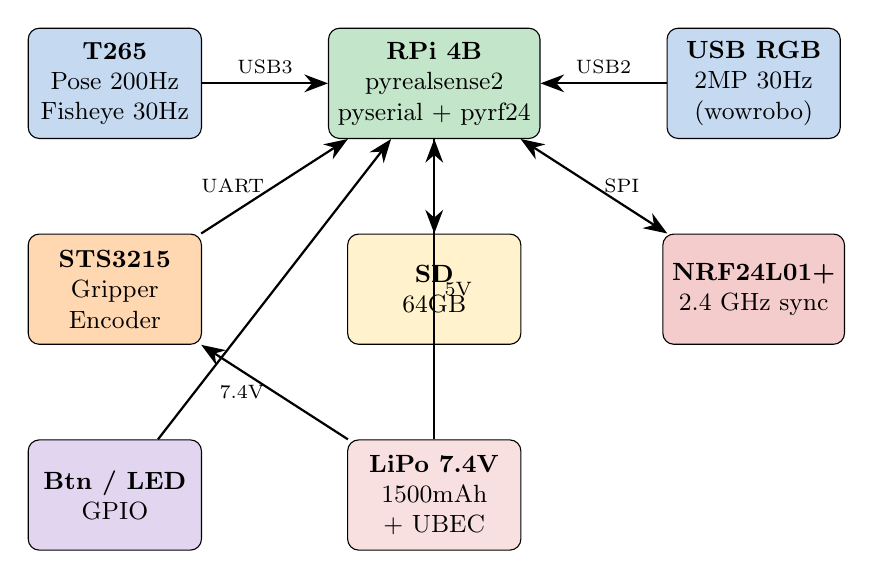
\begin{tikzpicture}[
  node distance=12mm and 16mm,
  every node/.style={draw, rounded corners=4pt, minimum width=22mm, minimum height=14mm, align=center, font=\small},
  arr/.style={-{Stealth[length=3mm]}, thick},
  biarr/.style={{Stealth[length=3mm]}-{Stealth[length=3mm]}, thick},
]
  % Row 0: sensors + compute
  \node[fill=nodeblue] (t265) {\textbf{T265}\\Pose 200Hz\\Fisheye 30Hz};
  \node[fill=nodegreen, right=of t265] (rpi) {\textbf{RPi 4B}\\pyrealsense2\\pyserial + pyrf24};
  \node[fill=nodeblue, right=of rpi] (rgb) {\textbf{USB RGB}\\2MP 30Hz\\(wowrobo)};

  % Row 1: actuator + storage + radio
  \node[fill=nodeorange, below=of t265] (servo) {\textbf{STS3215}\\Gripper\\Encoder};
  \node[fill=nodeyellow, below=of rpi] (sd) {\textbf{SD}\\64GB};
  \node[fill=nodered, below=of rgb] (nrf) {\textbf{NRF24L01+}\\2.4 GHz sync};

  % Row 2: UI + power
  \node[fill=nodepurple, below=of servo] (gpio) {\textbf{Btn / LED}\\GPIO};
  \node[fill=nodered!60!white, below=of sd] (pwr) {\textbf{LiPo 7.4V}\\1500mAh\\+ UBEC};

  % Edges
  \draw[arr] (t265) -- node[above, draw=none, minimum width=0, minimum height=0, font=\scriptsize]{USB3} (rpi);
  \draw[arr] (rgb) -- node[above, draw=none, minimum width=0, minimum height=0, font=\scriptsize]{USB2} (rpi);
  \draw[arr] (rpi) -- (sd);
  \draw[arr] (servo) -- node[left, draw=none, minimum width=0, minimum height=0, font=\scriptsize]{UART} (rpi);
  \draw[biarr] (nrf) -- node[right, draw=none, minimum width=0, minimum height=0, font=\scriptsize]{SPI} (rpi);
  \draw[arr] (gpio) -- (rpi);
  \draw[arr] (pwr) -- node[left, draw=none, minimum width=0, minimum height=0, font=\scriptsize]{7.4V} (servo);
  \draw[arr] (pwr) -- node[right, draw=none, minimum width=0, minimum height=0, font=\scriptsize]{5V} (rpi);
\end{tikzpicture}
\caption{Updated single gripper unit hardware architecture with NRF24L01+ radio and USB RGB camera (9 nodes). Total mass ${\sim}$360\,g, battery life ${\sim}$45\,min.}
\label{fig:hw-arch}
\end{figure}

\begin{table}[htbp]
\centering
\caption{Connection details for single gripper unit.}
\begin{tabular}{l l l l}
\toprule
\textbf{Connection} & \textbf{From} & \textbf{To} & \textbf{Notes} \\
\midrule
USB 3.0 & T265 Camera & RPi USB3 (blue) & Cable $<$ 30\,cm \\
USB 2.0 & wowrobo RGB & RPi USB2 & 3\,m cable \\
SPI + GPIO & NRF24L01+ & RPi SPI0 + GPIO22/25 & CE, CSN, IRQ \\
UART TX & RPi GPIO14 & STS3215 RX & 3.3V TTL \\
UART RX & RPi GPIO15 & STS3215 TX & 3.3V TTL \\
Power 7.4V & LiPo & STS3215 VCC & Direct connection \\
Power 5V & UBEC out & RPi USB-C & 5V 3A rated \\
Button & Switch & GPIO17 & Pull-up, active low \\
LED & GPIO27 & LED + resistor & 330$\Omega$ series \\
\bottomrule
\end{tabular}
\label{tab:connections}
\end{table}


% ─────────────────────────────────────────────────
% 2.2 NRF24L01+ Hardware
% ─────────────────────────────────────────────────
\subsection{NRF24L01+ Hardware}

The NRF24L01+ is a 2.4\,GHz ISM-band transceiver with hardware-accelerated Enhanced ShockBurst (ESB). It communicates with the RPi over SPI at up to 10\,MHz, and its 32-byte maximum payload is sufficient for our synchronization packet.

\subsubsection{Module Variants}

\begin{itemize}
  \item \textbf{Basic module} (green PCB, ${\sim}$\$1): On-board PCB antenna, 0\,dBm TX power, ${\sim}$10\,m indoor range. Draws 11.3\,mA at 0\,dBm, powered directly from RPi 3.3V pin.
  \item \textbf{PA+LNA module} (${\sim}$\$3): External antenna with power amplifier and low-noise amplifier, up to +20\,dBm TX, ${\sim}$100\,m indoor range. Draws up to 115\,mA at full power.
\end{itemize}

For bimanual grippers operating within ${\sim}$3\,m of each other, the basic module is sufficient.

\subsubsection{Pin Mapping}

\begin{table}[htbp]
\centering
\caption{NRF24L01+ to Raspberry Pi 4B GPIO pin mapping. Uses SPI0 bus.}
\begin{tabular}{l l l l l}
\toprule
\textbf{NRF Pin} & \textbf{Function} & \textbf{RPi GPIO} & \textbf{RPi Pin \#} & \textbf{Notes} \\
\midrule
VCC & Power & 3.3V & Pin 17 & Add 10\,$\mu$F + 100\,nF bypass \\
GND & Ground & GND & Pin 20 & \\
CE & Chip Enable & GPIO22 & Pin 15 & Active high: TX/RX enable \\
CSN & SPI Chip Select & GPIO8 (CE0) & Pin 24 & Active low: SPI select \\
SCK & SPI Clock & GPIO11 (SCLK) & Pin 23 & \\
MOSI & SPI Data In & GPIO10 (MOSI) & Pin 19 & \\
MISO & SPI Data Out & GPIO9 (MISO) & Pin 21 & \\
IRQ & Interrupt & GPIO25 & Pin 22 & Optional: active low \\
\bottomrule
\end{tabular}
\label{tab:nrf-pins}
\end{table}

\subsubsection{Wiring Schematic}

\begin{figure}[htbp]
\centering
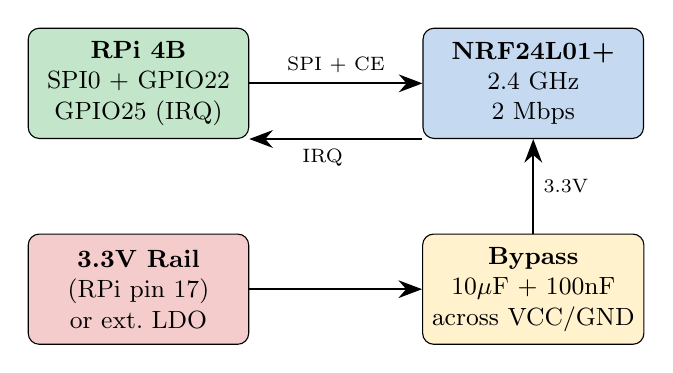
\begin{tikzpicture}[
  node distance=12mm and 20mm,
  every node/.style={draw, rounded corners=4pt, minimum width=28mm, minimum height=14mm, align=center, font=\small},
  arr/.style={-{Stealth[length=3mm]}, thick},
]
  \node[fill=nodegreen] (rpi) {\textbf{RPi 4B}\\SPI0 + GPIO22\\GPIO25 (IRQ)};
  \node[fill=nodeblue, right=22mm of rpi] (nrf) {\textbf{NRF24L01+}\\2.4 GHz\\2 Mbps};
  \node[fill=nodeyellow, below=of nrf] (cap) {\textbf{Bypass}\\10$\mu$F + 100nF\\across VCC/GND};
  \node[fill=nodered, below=of rpi] (pwr) {\textbf{3.3V Rail}\\(RPi pin 17)\\or ext.\ LDO};

  \draw[arr] (rpi) -- node[above, draw=none, minimum width=0, minimum height=0, font=\scriptsize]{SPI + CE} (nrf);
  \draw[arr] (nrf.south west) -- node[below left, draw=none, minimum width=0, minimum height=0, font=\scriptsize, pos=0.4]{IRQ} (rpi.south east);
  \draw[arr] (pwr) -- (cap);
  \draw[arr] (cap) -- node[right, draw=none, minimum width=0, minimum height=0, font=\scriptsize]{3.3V} (nrf);
\end{tikzpicture}
\caption{NRF24L01+ wiring to RPi 4B. Bypass capacitors are essential for stable operation.}
\label{fig:nrf-wiring}
\end{figure}

\begin{warningbox}[PA+LNA Power Warning]
The PA+LNA variant draws up to \textbf{115\,mA at full TX power}. The RPi 3.3V GPIO pin can supply only ${\sim}$50\,mA. Powering a PA+LNA module directly from the RPi 3.3V rail will cause voltage drops, SPI communication failures, and unreliable radio operation. Use an \textbf{AMS1117-3.3V LDO} fed from the 5V rail with 10\,$\mu$F input and output capacitors.
\end{warningbox}

\subsubsection{SPI Configuration}

Enable SPI on the Raspberry Pi:

\begin{lstlisting}[language=bash]
# Method 1: raspi-config
sudo raspi-config nonint do_spi 0

# Method 2: /boot/config.txt
# Add or uncomment: dtparam=spi=on

# Verify SPI is active
ls /dev/spidev0.*
# Should show: /dev/spidev0.0  /dev/spidev0.1
\end{lstlisting}

Install the pyRF24 library:

\begin{lstlisting}[language=bash]
pip install pyrf24
\end{lstlisting}


% ─────────────────────────────────────────────────
% 2.3 Bill of Materials
% ─────────────────────────────────────────────────
\subsection{Bill of Materials}

\begin{table}[htbp]
\centering
\caption{Updated BOM with NRF24L01+ and dual cameras (${\sim}$\$676 total).}
\begin{tabular}{l c r l}
\toprule
\textbf{Component} & \textbf{Qty} & \textbf{Cost} & \textbf{Note} \\
\midrule
Intel RealSense T265 & $\times$2 & ${\sim}$\$200 ea & eBay / AliExpress \\
Raspberry Pi 4B 4GB & $\times$2 & ${\sim}$\$55 ea & \\
MicroSD 64GB A2 & $\times$2 & ${\sim}$\$12 ea & High write speed \\
Feetech STS3215 & $\times$2 & ${\sim}$\$15 ea & 12-bit encoder \\
USB RGB Camera (wowrobo) & $\times$2 & ${\sim}$\$15 ea & 2MP, 30fps, 3m cable \\
NRF24L01+ module & $\times$2 & ${\sim}$\$1 ea & Basic PCB antenna \\
7.4V 2S LiPo 1500mAh & $\times$2 & ${\sim}$\$15 ea & XT30 + BMS \\
5V 3A UBEC & $\times$2 & ${\sim}$\$5 ea & \\
Misc + 3D housing & $\times$2 & ${\sim}$\$20 ea & PLA + TPU + caps \\
\midrule
\textbf{Bimanual total} & & \textbf{${\sim}$\$676} & \\
\bottomrule
\end{tabular}
\label{tab:bom}
\end{table}


% ─────────────────────────────────────────────────
% 2.4 Per-Gripper Software Architecture
% ─────────────────────────────────────────────────
\subsection{Per-Gripper Software Architecture}

Each RPi runs a single Python process with five threads feeding a synchronized buffer at 30\,Hz. The NRF sync trigger from Thread~4 serves as the master clock for frame assembly.

\begin{figure}[htbp]
\centering
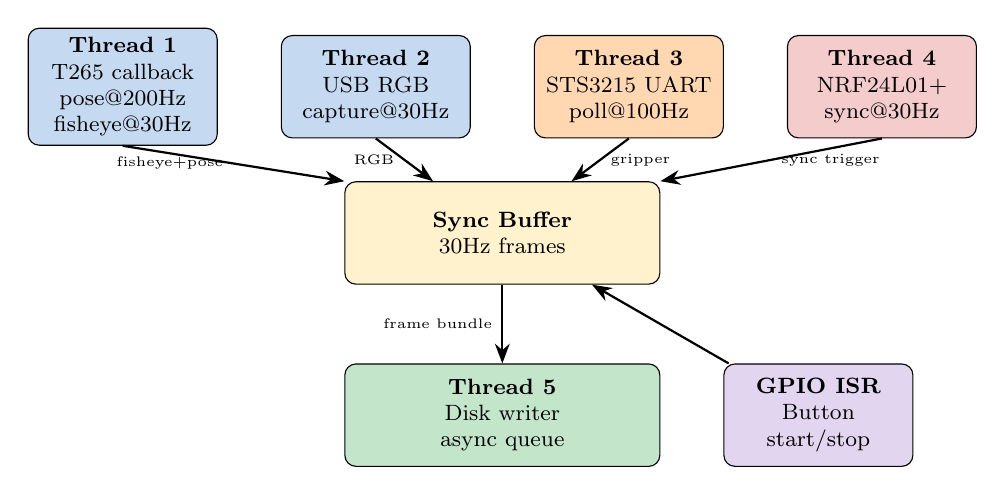
\begin{tikzpicture}[
  node distance=10mm and 12mm,
  every node/.style={draw, rounded corners=4pt, minimum width=24mm, minimum height=13mm, align=center, font=\footnotesize},
  arr/.style={-{Stealth[length=2.5mm]}, thick},
]
  % Thread row
  \node[fill=nodeblue] (t1) {\textbf{Thread 1}\\T265 callback\\pose@200Hz\\fisheye@30Hz};
  \node[fill=nodeblue, right=8mm of t1] (t2) {\textbf{Thread 2}\\USB RGB\\capture@30Hz};
  \node[fill=nodeorange, right=8mm of t2] (t3) {\textbf{Thread 3}\\STS3215 UART\\poll@100Hz};
  \node[fill=nodered, right=8mm of t3] (t4) {\textbf{Thread 4}\\NRF24L01+\\sync@30Hz};

  % Sync buffer
  \node[fill=nodeyellow, below=12mm of $(t2)!0.5!(t3)$, minimum width=40mm] (buf) {\textbf{Sync Buffer}\\30Hz frames};

  % Disk writer
  \node[fill=nodegreen, below=10mm of buf, minimum width=40mm] (t5) {\textbf{Thread 5}\\Disk writer\\async queue};

  % GPIO
  \node[fill=nodepurple, right=8mm of t5] (btn) {\textbf{GPIO ISR}\\Button\\start/stop};

  % Edges
  \draw[arr] (t1.south) -- node[left, draw=none, minimum width=0, minimum height=0, font=\tiny]{fisheye+pose} (buf.north west);
  \draw[arr] (t2.south) -- node[left, draw=none, minimum width=0, minimum height=0, font=\tiny]{RGB} (buf);
  \draw[arr] (t3.south) -- node[right, draw=none, minimum width=0, minimum height=0, font=\tiny]{gripper} (buf);
  \draw[arr] (t4.south) -- node[right, draw=none, minimum width=0, minimum height=0, font=\tiny]{sync trigger} (buf.north east);
  \draw[arr] (buf) -- node[left, draw=none, minimum width=0, minimum height=0, font=\tiny]{frame bundle} (t5);
  \draw[arr] (btn) -- (buf);
\end{tikzpicture}
\caption{Updated 5-thread software architecture. Thread~4 (NRF) provides the synchronization trigger; Thread~2 (USB RGB) adds color observation.}
\label{fig:sw-arch}
\end{figure}


% ─────────────────────────────────────────────────
% 2.5 Dual-Camera Integration
% ─────────────────────────────────────────────────
\subsection{Dual-Camera Integration}

Each gripper unit carries two cameras:

\begin{itemize}
  \item \textbf{Intel RealSense T265:} 6DoF VIO at 200\,Hz and fisheye stereo images at 30\,Hz. Connected via USB 3.0.
  \item \textbf{USB RGB Camera (wowrobo):} 2MP resolution, 30\,fps via USB 2.0 with 3\,m cable. Designed for SO-ARM100/101 integration.
\end{itemize}

\begin{table}[htbp]
\centering
\caption{Dual camera specifications per gripper unit.}
\begin{tabular}{l c c c l}
\toprule
\textbf{Camera} & \textbf{Resolution} & \textbf{FPS} & \textbf{FOV} & \textbf{Purpose} \\
\midrule
T265 (fisheye) & 848$\times$800 & 30 & 163$^\circ$ & Wide-angle observation + VIO pose \\
wowrobo RGB & 1920$\times$1080 & 30 & ${\sim}$78$^\circ$ & Close-range color observation \\
\bottomrule
\end{tabular}
\label{tab:cameras}
\end{table}

\begin{infobox}[USB Bandwidth Budget]
The RPi 4B has separate USB 3.0 (VL805) and USB 2.0 controllers. The T265 uses USB~3.0 (${\sim}$200\,MB/s available). The wowrobo RGB camera uses USB~2.0 (${\sim}$40\,MB/s available; 1080p MJPEG@30fps needs ${\sim}$15\,MB/s). The NRF24L01+ uses SPI (separate from USB entirely). No bandwidth conflicts exist.
\end{infobox}


% ════════════════════════════════════════════════════════════
% 3. Enhanced ShockBurst Protocol
% ════════════════════════════════════════════════════════════
\section{Enhanced ShockBurst Protocol}

The NRF24L01+ implements \textbf{Enhanced ShockBurst} (ESB), a hardware-accelerated packet protocol that handles preamble generation, address matching, CRC validation, automatic acknowledgement, and retransmission---all in silicon, without CPU intervention.

% ─────────────────────────────────────────────────
% 3.1 On-Air Packet Format
% ─────────────────────────────────────────────────
\subsection{On-Air Packet Format}

\begin{figure}[htbp]
\centering
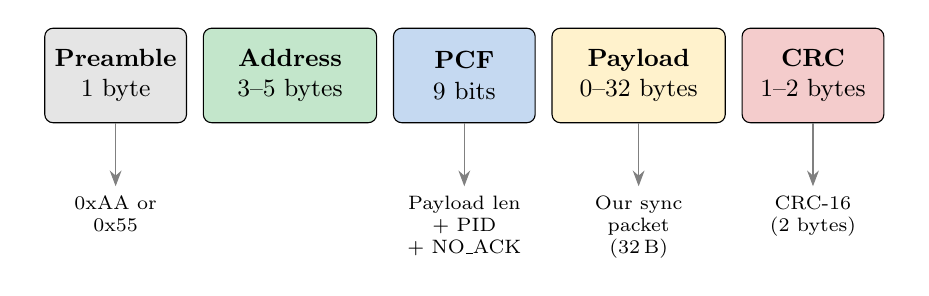
\begin{tikzpicture}[
  box/.style={draw, rounded corners=3pt, minimum height=12mm, align=center, font=\small},
  ann/.style={font=\scriptsize, align=center, text width=20mm},
  arr/.style={-{Stealth[length=2mm]}, gray},
]
  \node[box, fill=black!10, minimum width=18mm] (pre) at (0,0) {\textbf{Preamble}\\1 byte};
  \node[box, fill=nodegreen, minimum width=22mm, right=2mm of pre] (addr) {\textbf{Address}\\3--5 bytes};
  \node[box, fill=nodeblue, minimum width=18mm, right=2mm of addr] (pcf) {\textbf{PCF}\\9 bits};
  \node[box, fill=nodeyellow, minimum width=22mm, right=2mm of pcf] (pay) {\textbf{Payload}\\0--32 bytes};
  \node[box, fill=nodered, minimum width=18mm, right=2mm of pay] (crc) {\textbf{CRC}\\1--2 bytes};

  % Annotations
  \node[ann, below=8mm of pre] (pn) {0xAA or\\0x55};
  \node[ann, below=8mm of pcf] (pcfn) {Payload len\\+ PID\\+ NO\_ACK};
  \node[ann, below=8mm of pay] (payn) {Our sync\\packet\\(32\,B)};
  \node[ann, below=8mm of crc] (crcn) {CRC-16\\(2 bytes)};

  \draw[arr] (pre.south) -- (pn.north);
  \draw[arr] (pcf.south) -- (pcfn.north);
  \draw[arr] (pay.south) -- (payn.north);
  \draw[arr] (crc.south) -- (crcn.north);
\end{tikzpicture}
\caption{ESB on-air packet format. The Packet Control Field (PCF) is 9 bits packed before the payload.}
\label{fig:esb-packet}
\end{figure}

% ─────────────────────────────────────────────────
% 3.2 PCF Breakdown
% ─────────────────────────────────────────────────
\subsection{PCF Breakdown}

\begin{table}[htbp]
\centering
\caption{PCF field breakdown. PID increments per new payload to detect retransmitted duplicates.}
\begin{tabular}{l c l l}
\toprule
\textbf{Field} & \textbf{Bits} & \textbf{Range} & \textbf{Purpose} \\
\midrule
Payload Length & 6 & 0--32 & Dynamic payload size in bytes \\
PID & 2 & 0--3 & Packet ID for duplicate detection \\
NO\_ACK & 1 & 0/1 & Per-packet ACK disable flag \\
\bottomrule
\end{tabular}
\label{tab:pcf}
\end{table}

% ─────────────────────────────────────────────────
% 3.3 Auto-ACK and Retransmission
% ─────────────────────────────────────────────────
\subsection{Auto-ACK and Retransmission}

When Enhanced ShockBurst is enabled (default), the transmitter automatically:

\begin{enumerate}
  \item Sends the packet and switches to RX mode
  \item Waits for an ACK from the receiver within the \textbf{Auto Retransmit Delay} (ARD)
  \item If no ACK is received, retransmits up to \textbf{ARC} times (configurable 0--15)
  \item Reports success or max-retries-exceeded to the application
\end{enumerate}

The receiver, upon validating address and CRC, automatically sends an ACK packet. The PID field prevents the receiver from delivering duplicate payloads caused by ACK packets lost on the return path.

% ─────────────────────────────────────────────────
% 3.4 ESB Timing
% ─────────────────────────────────────────────────
\subsection{ESB Timing}

\begin{table}[htbp]
\centering
\caption{ESB timing for a single transmission at 2\,Mbps with 32-byte payload.}
\begin{tabular}{l c c c c c}
\toprule
 & PLL Lock & TX Packet & RX Switch & Wait ACK & ACK RX \\
\midrule
\textbf{Duration} & \cellcolor{nodeblue}130\,$\mu$s & \cellcolor{nodegreen}164.5\,$\mu$s & \cellcolor{nodeorange}${\sim}$10\,$\mu$s & \cellcolor{nodeyellow}ARD & \cellcolor{nodeblue}${\sim}$30\,$\mu$s \\
\textbf{State} & \cellcolor{nodeblue}Standby & \cellcolor{nodegreen}TX & \cellcolor{nodeorange}TX$\to$RX & \cellcolor{nodeyellow}RX & \cellcolor{nodeblue}RX \\
\bottomrule
\end{tabular}
\label{tab:esb-timing}
\end{table}

% ─────────────────────────────────────────────────
% 3.5 Data Rate Selection
% ─────────────────────────────────────────────────
\subsection{Data Rate Selection}

\begin{table}[htbp]
\centering
\caption{Data rate comparison. We use 2\,Mbps to minimize radio-on time and latency.}
\begin{tabular}{l c c l}
\toprule
\textbf{Data Rate} & \textbf{32B TX Time} & \textbf{On-Air Time} & \textbf{Use Case} \\
\midrule
250 kbps & ${\sim}$1.3\,ms & ${\sim}$1.5\,ms & Maximum range, lowest throughput \\
1 Mbps & ${\sim}$0.33\,ms & ${\sim}$0.5\,ms & Balanced \\
\textbf{2 Mbps} & \textbf{${\sim}$0.16\,ms} & \textbf{${\sim}$0.35\,ms} & \textbf{Minimum latency (our choice)} \\
\bottomrule
\end{tabular}
\label{tab:data-rates}
\end{table}

We select \textbf{2\,Mbps} because our payloads are small (32 bytes) and range requirements are modest (${\sim}$3\,m between grippers). The shorter on-air time also reduces collision probability in the crowded 2.4\,GHz band.

% ─────────────────────────────────────────────────
% 3.6 ACK Payload Feature
% ─────────────────────────────────────────────────
\subsection{ACK Payload Feature}

A key feature for our protocol: the receiver can \textbf{pre-load a payload into the ACK packet}. When the transmitter sends a packet and the receiver auto-ACKs, the ACK carries the pre-loaded data back. This enables bidirectional data exchange in a single radio transaction---critical for low-latency time synchronization.

The ACK payload must be loaded \emph{before} the TX packet arrives. The ACK payload can be up to 32 bytes, same as a normal payload.

\begin{infobox}[Channel Selection]
The NRF24L01+ operates on channels 0--125 (2400--2525\,MHz). WiFi channels 1, 6, and 11 occupy 2401--2473\,MHz. To avoid interference, we use \textbf{channel 108} (2508\,MHz), which is above the WiFi band.
\end{infobox}


% ════════════════════════════════════════════════════════════
% 4. Bimanual Synchronization
% ════════════════════════════════════════════════════════════
\section{Bimanual Synchronization}

% ─────────────────────────────────────────────────
% 4.1 Problem: Clock Drift
% ─────────────────────────────────────────────────
\subsection{Problem: Clock Drift}

If each RPi runs \texttt{sleep(1/30)} independently, Linux scheduler jitter (${\sim}$4\,$\mu$s/step) accumulates:

\begin{equation}
\Delta t(n) = \sum_{i=1}^{n}(T_A^i - T_B^i) \approx n \cdot 4\,\mu\text{s}
\label{eq:drift}
\end{equation}

After 5 minutes (9000 steps): \textbf{36\,ms drift}---more than one full 33\,ms frame.

% ─────────────────────────────────────────────────
% 4.2 Ping-Pong Protocol Design
% ─────────────────────────────────────────────────
\subsection{Ping-Pong Protocol Design}

Time synchronization requires bidirectional communication. The NRF24L01+ offers two approaches.

\subsubsection{Approach 1: Software Ping-Pong}

In software ping-pong, each peer explicitly switches between TX and RX modes:

\begin{figure}[htbp]
\centering
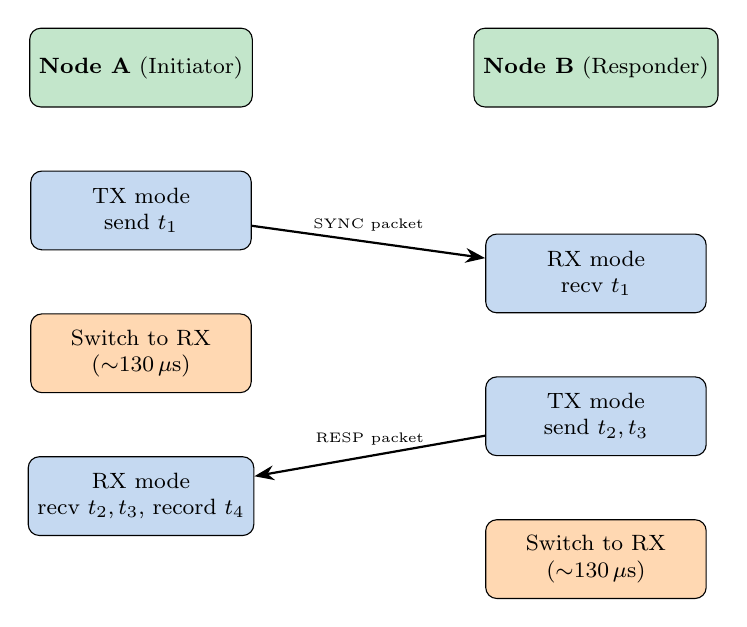
\begin{tikzpicture}[
  node distance=5mm and 28mm,
  every node/.style={draw, rounded corners=4pt, minimum width=28mm, minimum height=10mm, align=center, font=\footnotesize},
  arr/.style={-{Stealth[length=2.5mm]}, thick},
]
  % Headers
  \node[fill=nodegreen] (ha) {\textbf{Node A} (Initiator)};
  \node[fill=nodegreen, right=28mm of ha] (hb) {\textbf{Node B} (Responder)};

  % Step 1
  \node[fill=nodeblue, below=8mm of ha] (a1) {TX mode\\send $t_1$};
  \node[fill=nodeblue, below=16mm of hb] (b1) {RX mode\\recv $t_1$};
  \draw[arr] (a1) -- node[above, draw=none, minimum width=0, minimum height=0, font=\tiny]{SYNC packet} (b1);

  % Step 2
  \node[fill=nodeorange, below=8mm of a1] (a2) {Switch to RX\\(${\sim}$130\,$\mu$s)};

  % Step 3
  \node[fill=nodeblue, below=8mm of b1] (b2) {TX mode\\send $t_2, t_3$};
  \node[fill=nodeblue, below=8mm of a2] (a3) {RX mode\\recv $t_2, t_3$, record $t_4$};
  \draw[arr] (b2) -- node[above, draw=none, minimum width=0, minimum height=0, font=\tiny]{RESP packet} (a3);

  % Step 4
  \node[fill=nodeorange, below=8mm of b2] (b3) {Switch to RX\\(${\sim}$130\,$\mu$s)};
\end{tikzpicture}
\caption{Software ping-pong: 4 mode switches per round trip. Each switch adds ${\sim}$130\,$\mu$s PLL lock time.}
\label{fig:sw-pingpong}
\end{figure}

\subsubsection{Approach 2: Hardware ACK Payload}

The ACK payload feature eliminates explicit mode switching. Node~B pre-loads its response data into the ACK payload buffer. When Node~A transmits, hardware automatically sends an ACK containing Node~B's data.

\begin{figure}[htbp]
\centering
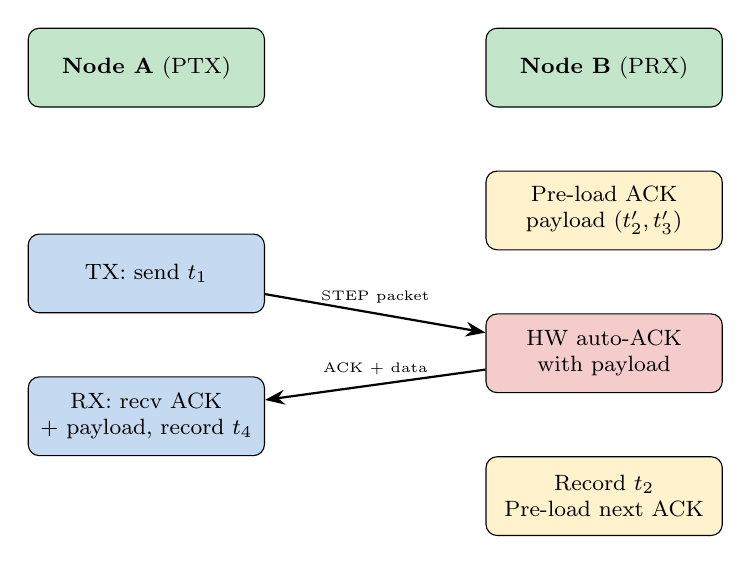
\begin{tikzpicture}[
  node distance=5mm and 28mm,
  every node/.style={draw, rounded corners=4pt, minimum width=30mm, minimum height=10mm, align=center, font=\footnotesize},
  arr/.style={-{Stealth[length=2.5mm]}, thick},
]
  % Headers
  \node[fill=nodegreen] (ha) {\textbf{Node A} (PTX)};
  \node[fill=nodegreen, right=28mm of ha] (hb) {\textbf{Node B} (PRX)};

  % Pre-load
  \node[fill=nodeyellow, below=8mm of hb] (pre) {Pre-load ACK\\payload ($t_2', t_3'$)};

  % TX
  \node[fill=nodeblue, below=16mm of ha] (tx) {TX: send $t_1$};
  \node[fill=nodered, below=8mm of pre] (ack) {HW auto-ACK\\with payload};
  \node[fill=nodeblue, below=8mm of tx] (rx) {RX: recv ACK\\+ payload, record $t_4$};

  \draw[arr] (tx) -- node[above, draw=none, minimum width=0, minimum height=0, font=\tiny]{STEP packet} (ack);
  \draw[arr] (ack) -- node[above, draw=none, minimum width=0, minimum height=0, font=\tiny]{ACK + data} (rx);

  % B updates
  \node[fill=nodeyellow, below=8mm of ack] (upd) {Record $t_2$\\Pre-load next ACK};
\end{tikzpicture}
\caption{Hardware ACK payload: zero explicit mode switches. Node~B stays in PRX mode permanently.}
\label{fig:hw-ack}
\end{figure}

\begin{table}[htbp]
\centering
\caption{Comparison of ping-pong approaches. We use hardware ACK payload for lower latency.}
\begin{tabular}{l c c}
\toprule
\textbf{Property} & \textbf{Software Ping-Pong} & \textbf{HW ACK Payload} \\
\midrule
Mode switches / round & 4 & 0 (hardware) \\
Round-trip time & ${\sim}$1.5\,ms & ${\sim}$0.6\,ms \\
Implementation complexity & Medium & Low \\
Timestamp freshness & Current round & Previous round \\
Payload size each way & 32\,B & 32\,B \\
\bottomrule
\end{tabular}
\label{tab:pingpong-compare}
\end{table}

We choose the \textbf{hardware ACK payload} approach. The one-round timestamp staleness (33\,ms at 30\,Hz) introduces negligible error: at 20\,ppm clock drift, 33\,ms contributes only 0.66\,ns of additional offset.

% ─────────────────────────────────────────────────
% 4.3 Bimanual Topology
% ─────────────────────────────────────────────────
\subsection{Bimanual Topology}

\begin{figure}[htbp]
\centering
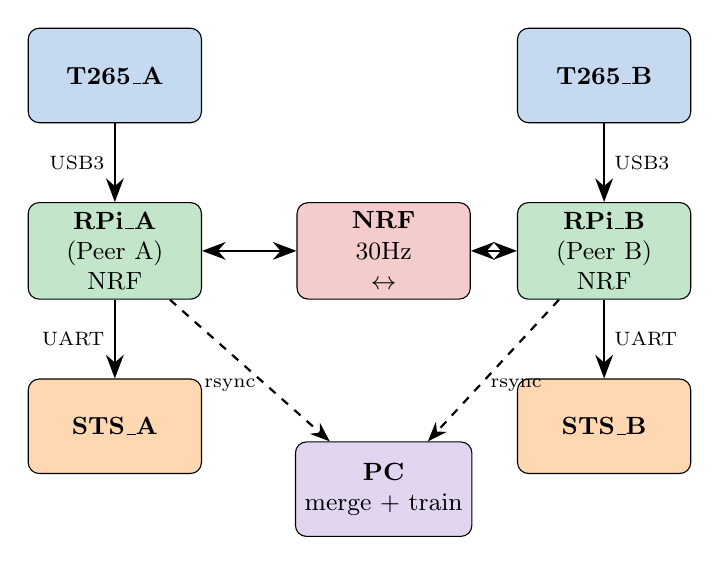
\begin{tikzpicture}[
  node distance=10mm and 16mm,
  every node/.style={draw, rounded corners=4pt, minimum width=22mm, minimum height=12mm, align=center, font=\small},
  arr/.style={-{Stealth[length=3mm]}, thick},
  biarr/.style={{Stealth[length=3mm]}-{Stealth[length=3mm]}, thick},
  darr/.style={-{Stealth[length=2.5mm]}, thick, dashed},
]
  % Peer A (Left)
  \node[fill=nodeblue] (tl) {\textbf{T265\_A}};
  \node[fill=nodegreen, below=of tl] (rl) {\textbf{RPi\_A}\\(Peer A)\\NRF};
  \node[fill=nodeorange, below=of rl] (sl) {\textbf{STS\_A}};

  % Peer B (Right)
  \node[fill=nodeblue, right=40mm of tl] (tr) {\textbf{T265\_B}};
  \node[fill=nodegreen, below=of tr] (rr) {\textbf{RPi\_B}\\(Peer B)\\NRF};
  \node[fill=nodeorange, below=of rr] (sr) {\textbf{STS\_B}};

  % Sync link
  \node[fill=nodered, right=12mm of rl] (nrf) {\textbf{NRF}\\30Hz\\$\leftrightarrow$};

  % PC
  \node[fill=nodepurple, below=18mm of nrf] (pc) {\textbf{PC}\\merge + train};

  % Edges
  \draw[arr] (tl) -- node[left, draw=none, minimum width=0, minimum height=0, font=\scriptsize]{USB3} (rl);
  \draw[arr] (rl) -- node[left, draw=none, minimum width=0, minimum height=0, font=\scriptsize]{UART} (sl);
  \draw[arr] (tr) -- node[right, draw=none, minimum width=0, minimum height=0, font=\scriptsize]{USB3} (rr);
  \draw[arr] (rr) -- node[right, draw=none, minimum width=0, minimum height=0, font=\scriptsize]{UART} (sr);
  \draw[biarr] (rl) -- (nrf);
  \draw[biarr] (nrf) -- (rr);
  \draw[darr] (rl) -- node[left, draw=none, minimum width=0, minimum height=0, font=\scriptsize, pos=0.6]{rsync} (pc);
  \draw[darr] (rr) -- node[right, draw=none, minimum width=0, minimum height=0, font=\scriptsize, pos=0.6]{rsync} (pc);
\end{tikzpicture}
\caption{Bimanual topology with symmetric NRF peers. Both grippers communicate bidirectionally via NRF24L01+ ESB.}
\label{fig:bimanual-topo}
\end{figure}

% ─────────────────────────────────────────────────
% 4.4 Time Sync Algorithm
% ─────────────────────────────────────────────────
\subsection{Time Sync Algorithm}

\subsubsection{NTP-Style Four-Timestamp Principle}

Clock synchronization between two peers requires estimating the \textbf{offset} $\theta$ between their clocks and the \textbf{one-way delay} $\delta$. Using four timestamps from a single round trip:

\begin{figure}[htbp]
\centering
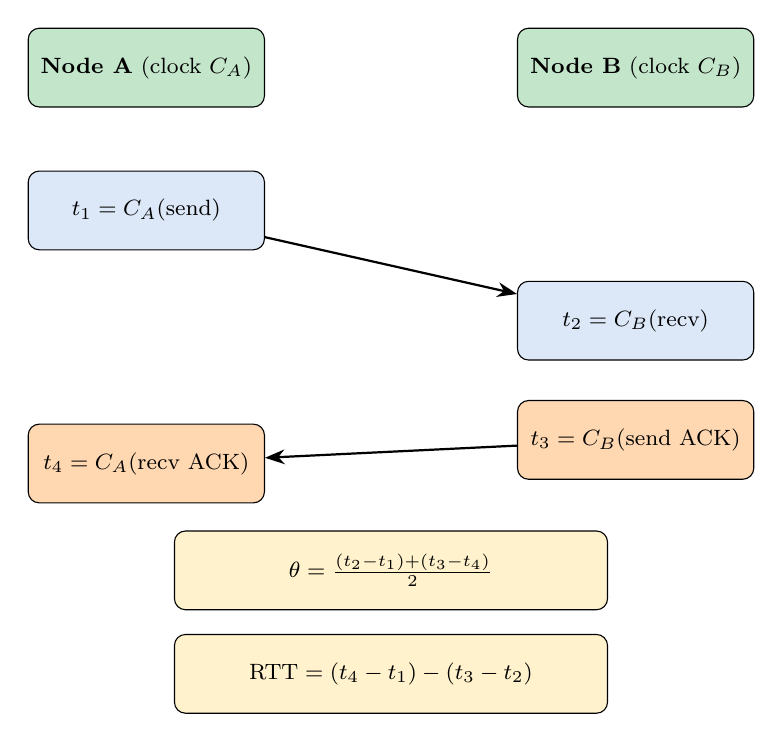
\begin{tikzpicture}[
  node distance=5mm and 32mm,
  every node/.style={draw, rounded corners=4pt, minimum width=30mm, minimum height=10mm, align=center, font=\footnotesize},
  arr/.style={-{Stealth[length=2.5mm]}, thick},
]
  % Headers
  \node[fill=nodegreen] (ca) {\textbf{Node A} (clock $C_A$)};
  \node[fill=nodegreen, right=32mm of ca] (cb) {\textbf{Node B} (clock $C_B$)};

  % Timestamps
  \node[fill=nodeblue!60!white, below=8mm of ca] (t1) {$t_1 = C_A(\text{send})$};
  \node[fill=nodeblue!60!white, below=22mm of cb] (t2) {$t_2 = C_B(\text{recv})$};
  \node[fill=nodeorange, below=5mm of t2] (t3) {$t_3 = C_B(\text{send ACK})$};
  \node[fill=nodeorange, below=22mm of t1] (t4) {$t_4 = C_A(\text{recv ACK})$};

  \draw[arr] (t1) -- (t2);
  \draw[arr] (t3) -- (t4);

  % Results
  \node[fill=nodeyellow, below=10mm of $(t4)!0.5!(t3)$, minimum width=55mm] (off) {$\theta = \frac{(t_2 - t_1) + (t_3 - t_4)}{2}$};
  \node[fill=nodeyellow, below=3mm of off, minimum width=55mm] (rtt) {$\text{RTT} = (t_4 - t_1) - (t_3 - t_2)$};
\end{tikzpicture}
\caption{Four-timestamp exchange. $t_1, t_4$ measured on Node A's clock; $t_2, t_3$ on Node B's clock.}
\label{fig:four-timestamp}
\end{figure}

\subsubsection{Mathematical Derivation}

Let $\theta = C_B - C_A$ be the true clock offset (B ahead of A) and assume symmetric one-way delay $d$:

\begin{equation}
t_2 = t_1 + d + \theta \qquad\qquad t_4 = t_3 + d - \theta
\end{equation}

Solving for $\theta$:

\begin{equation}
\theta = \frac{(t_2 - t_1) + (t_3 - t_4)}{2}
\label{eq:offset}
\end{equation}

The round-trip time (network delay only, excluding processing):

\begin{equation}
\text{RTT} = (t_4 - t_1) - (t_3 - t_2)
\label{eq:rtt}
\end{equation}

\subsubsection{Multi-Round Averaging with Outlier Rejection}

A single round provides one offset estimate, but Linux scheduling jitter can cause individual measurements to be noisy. We perform \textbf{10 rounds} and use median-based outlier rejection:

\begin{enumerate}
  \item Collect 10 $(\theta_i, \text{RTT}_i)$ pairs
  \item Compute $\tilde{\text{RTT}} = \text{median}(\text{RTT}_1, \ldots, \text{RTT}_{10})$
  \item Discard any round where $\text{RTT}_i > 1.5 \cdot \tilde{\text{RTT}}$ (jitter outlier)
  \item Final offset $\hat{\theta} = \text{mean}(\theta_i \text{ for kept rounds})$
\end{enumerate}

\subsubsection{Synchronization Algorithm (Pseudocode)}

\begin{figure}[htbp]
\begin{algorithm}[H]
\SetAlgoLined
\SetKwInOut{Input}{Input}
\SetKwInOut{Output}{Output}
\Input{radio (configured RF24), num\_rounds $= 10$}
\Output{clock offset $\hat{\theta}$, mean RTT}
offsets $\leftarrow []$, rtts $\leftarrow []$\;
\For{$i \leftarrow 1$ \KwTo num\_rounds}{
  build SYNC packet with $t_1 \leftarrow \texttt{monotonic()}$\;
  \texttt{radio.write(packet)} \tcp*{TX + wait for ACK payload}
  $t_4 \leftarrow \texttt{monotonic()}$\;
  parse ACK payload: extract $t_2, t_3$\;
  $\theta_i \leftarrow \frac{(t_2 - t_1) + (t_3 - t_4)}{2}$\;
  $\text{RTT}_i \leftarrow (t_4 - t_1) - (t_3 - t_2)$\;
  append $\theta_i$ to offsets, $\text{RTT}_i$ to rtts\;
  \texttt{sleep(5\,ms)} \tcp*{allow responder to pre-load next ACK}
}
$\tilde{\text{RTT}} \leftarrow \texttt{median(rtts)}$\;
\ForEach{$(\theta_i, \text{RTT}_i)$}{
  \If{$\text{RTT}_i > 1.5 \cdot \tilde{\text{RTT}}$}{discard $\theta_i$}
}
$\hat{\theta} \leftarrow \texttt{mean(kept\ offsets)}$\;
\Return $\hat{\theta}$, $\texttt{mean(kept\ RTTs)}$\;
\caption{Time Synchronization --- Initiator (Node A)}
\label{alg:time-sync}
\end{algorithm}
\end{figure}

\subsubsection{Worked Numerical Example}

\begin{table}[htbp]
\centering
\caption{Worked example with 5 rounds. Median RTT = 0.80\,ms, threshold = 1.20\,ms. Round~3 rejected.}
\begin{tabular}{c r r r r c}
\toprule
\textbf{Round} & $t_2{-}t_1$ (ms) & $t_3{-}t_4$ (ms) & $\theta_i$ (ms) & RTT (ms) & \textbf{Keep?} \\
\midrule
1 & 0.42 & $-0.38$ & 0.020 & 0.80 & \checkmark \\
2 & 0.41 & $-0.39$ & 0.010 & 0.80 & \checkmark \\
3 & 0.85 & $-0.37$ & 0.240 & 1.22 & $\times$ \\
4 & 0.43 & $-0.40$ & 0.015 & 0.83 & \checkmark \\
5 & 0.40 & $-0.38$ & 0.010 & 0.78 & \checkmark \\
\midrule
\textbf{Result} & & & \textbf{0.014} & \textbf{0.80} & \\
\bottomrule
\end{tabular}
\label{tab:worked-example}
\end{table}

\begin{warningbox}[Use Monotonic Clock]
Always use \texttt{time.monotonic()} (Python) or \texttt{CLOCK\_MONOTONIC} (C). The wall clock \texttt{time.time()} can jump due to NTP adjustments. A jump of even 1\,ms during a sync round would corrupt the offset estimate. \texttt{time.monotonic()} is immune to these adjustments and has nanosecond resolution on Linux.
\end{warningbox}

% ─────────────────────────────────────────────────
% 4.5 Alternating Triggers
% ─────────────────────────────────────────────────
\subsection{Alternating Triggers}

During recording, peers alternate sending step triggers, ensuring symmetric latency distribution:

\begin{equation}
\Delta t(n) = \tau_{\text{NRF}} \approx 0.8\,\text{ms} \quad \forall\, n
\label{eq:bounded}
\end{equation}

\begin{figure}[htbp]
\centering
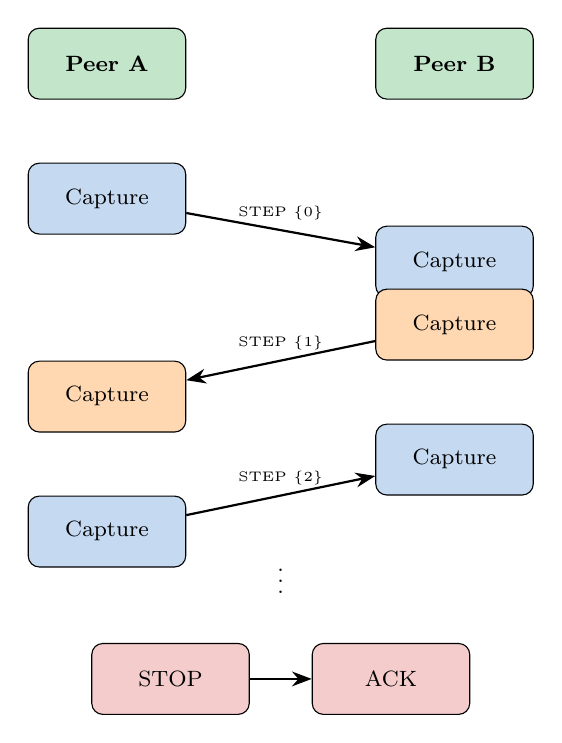
\begin{tikzpicture}[
  node distance=5mm and 24mm,
  every node/.style={draw, rounded corners=4pt, minimum width=20mm, minimum height=9mm, align=center, font=\footnotesize},
  arr/.style={-{Stealth[length=2.5mm]}, thick},
]
  % Headers
  \node[fill=nodegreen] (ha) {\textbf{Peer A}};
  \node[fill=nodegreen, right=24mm of ha] (hb) {\textbf{Peer B}};

  % Step 0 (even -> A triggers)
  \node[fill=nodeblue, below=8mm of ha] (a0) {Capture};
  \node[fill=nodeblue, below=16mm of hb] (b0) {Capture};
  \draw[arr] (a0) -- node[above, draw=none, minimum width=0, minimum height=0, font=\tiny]{STEP \{0\}} (b0);

  % Step 1 (odd -> B triggers)
  \node[fill=nodeorange, below=8mm of hb, yshift=-16mm] (b1) {Capture};
  \node[fill=nodeorange, below=8mm of a0, yshift=-8mm] (a1) {Capture};
  \draw[arr] (b1) -- node[above, draw=none, minimum width=0, minimum height=0, font=\tiny]{STEP \{1\}} (a1);

  % Step 2 (even -> A triggers)
  \node[fill=nodeblue, below=8mm of a1] (a2) {Capture};
  \node[fill=nodeblue, below=8mm of b1] (b2) {Capture};
  \draw[arr] (a2) -- node[above, draw=none, minimum width=0, minimum height=0, font=\tiny]{STEP \{2\}} (b2);

  % Dots
  \node[draw=none, below=6mm of $(a2)!0.5!(b2)$, minimum width=0, minimum height=0] (dots) {$\vdots$};

  % Stop
  \node[fill=nodered, below=5mm of dots, xshift=-14mm] (sa) {STOP};
  \node[fill=nodered, below=5mm of dots, xshift=14mm] (sb) {ACK};
  \draw[arr] (sa) -- (sb);
\end{tikzpicture}
\caption{Alternating trigger protocol. Even steps (blue): Peer~A captures first. Odd steps (orange): Peer~B captures first. This ensures symmetric average latency.}
\label{fig:alt-triggers}
\end{figure}

\begin{table}[htbp]
\centering
\caption{Error comparison. Independent loop grows linearly; NRF trigger stays constant.}
\begin{tabular}{l r r c}
\toprule
\textbf{Duration} & \textbf{Steps} & \textbf{Independent} & \textbf{NRF} \\
\midrule
3 s & 100 & 0.4\,ms & ${\sim}$0.8\,ms \\
30 s & 1k & 4\,ms & ${\sim}$0.8\,ms \\
100 s & 3k & 12\,ms & ${\sim}$0.8\,ms \\
5 min & 9k & 36\,ms & ${\sim}$0.8\,ms \\
\bottomrule
\end{tabular}
\label{tab:error-compare}
\end{table}

% ─────────────────────────────────────────────────
% 4.6 NRF Packet Format
% ─────────────────────────────────────────────────
\subsection{NRF Packet Format}

We use a 32-byte NRF packet, filling the maximum payload exactly:

\begin{table}[htbp]
\centering
\caption{32-byte NRF packet format. Extended from 28-byte UDP with seq\_num and reserved bytes.}
\begin{tabular}{l l r l l}
\toprule
\textbf{Field} & \textbf{Type} & \textbf{Size} & \textbf{Offset} & \textbf{Role} \\
\midrule
magic & char[2] & 2\,B & 0 & ``GS'' identifier \\
msg\_type & uint8 & 1\,B & 2 & SYNC/STEP/STOP/ACK \\
step & uint32 & 4\,B & 3 & Absolute step number \\
episode & uint16 & 2\,B & 7 & Episode index \\
flags & uint8 & 1\,B & 9 & REC / PAUSE / RESYNC \\
sender\_id & uint8 & 1\,B & 10 & Peer A=0, B=1 \\
timestamp & float64 & 8\,B & 11 & Sender monotonic clock (s) \\
sync\_t2 & float64 & 8\,B & 19 & Responder recv timestamp \\
seq\_num & uint8 & 1\,B & 27 & Sequence counter (0--255) \\
reserved & uint8[3] & 3\,B & 28 & Future use / padding \\
checksum & uint8 & 1\,B & 31 & XOR of bytes 0--30 \\
\midrule
 & & \textbf{32\,B} & & \\
\bottomrule
\end{tabular}
\label{tab:nrf-packet}
\end{table}

\begin{infobox}[Payload Size Trade-Off]
The existing UDP protocol uses 28 bytes. Adding a sequence number (1\,B) and keeping 3\,B reserved for future extensions fills the 32-byte NRF maximum exactly. Since NRF24L01+ charges the same air time for any payload up to 32 bytes when using dynamic payloads, there is no penalty for using the full capacity.
\end{infobox}

% ─────────────────────────────────────────────────
% 4.7 Timing Waveform
% ─────────────────────────────────────────────────
\subsection{Timing Waveform}

\begin{table}[htbp]
\centering
\caption{Timing diagram showing alternating triggers. NRF latency ${\sim}$0.8\,ms.}
\setlength{\tabcolsep}{4pt}
\begin{tabular}{l *{8}{c}}
\toprule
 & 0 & 1 & 2 & 3 & 4 & 5 & 6 & 7 \\
\midrule
\textbf{A capture} & \cellcolor{nodeblue}\checkmark & \cellcolor{nodeblue}\checkmark & & & \cellcolor{nodeblue}\checkmark & \cellcolor{nodeblue}\checkmark & & \\
\textbf{A$\to$B} & & \cellcolor{nodegreen}$\to$ & \cellcolor{nodegreen}$\to$ & & & \cellcolor{nodegreen}$\to$ & \cellcolor{nodegreen}$\to$ & \\
\textbf{B capture} & & & \cellcolor{nodeorange}\checkmark & \cellcolor{nodeorange}\checkmark & & \cellcolor{nodeorange}\checkmark & \cellcolor{nodeorange}\checkmark & \\
\textbf{B$\to$A} & & & & \cellcolor{nodegreen}$\leftarrow$ & \cellcolor{nodegreen}$\leftarrow$ & & & \cellcolor{nodegreen}$\leftarrow$ \\
\midrule
\textbf{Step} & & \cellcolor{nodeblue!30}0 & & \cellcolor{nodeorange!30}1 & & \cellcolor{nodeblue!30}2 & & \\
\bottomrule
\end{tabular}
\label{tab:timing-waveform}
\end{table}


% ════════════════════════════════════════════════════════════
% 5. Error Handling
% ════════════════════════════════════════════════════════════
\section{Error Handling}

% ─────────────────────────────────────────────────
% 5.1 Packet Loss Scenarios
% ─────────────────────────────────────────────────
\subsection{Packet Loss Scenarios}

Three failure tiers:

\begin{enumerate}
  \item \textbf{Transient loss:} 1--2 packets lost, ESB auto-retry succeeds. Invisible to application. Adds ${\sim}$0.5\,ms per retry to RTT.
  \item \textbf{Burst loss:} 3+ consecutive packets lost despite 15 retries. Software timeout fires (200\,ms). Insert empty frame(s) and continue.
  \item \textbf{Persistent failure:} 3 consecutive software timeouts. Enter RESYNC state, re-run time synchronization, resume recording.
\end{enumerate}

% ─────────────────────────────────────────────────
% 5.2 Protocol State Machine
% ─────────────────────────────────────────────────
\subsection{Protocol State Machine}

\begin{figure}[htbp]
\centering
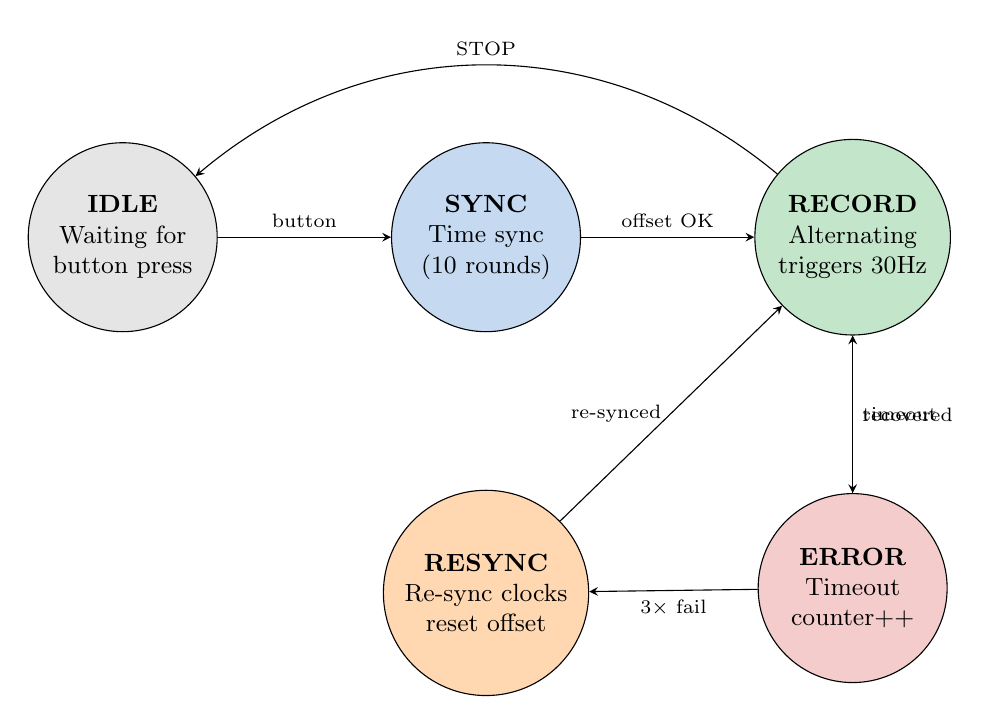
\begin{tikzpicture}[
  ->,>=stealth,
  node distance=20mm and 22mm,
  every state/.style={draw, rounded corners=4pt, minimum width=24mm, minimum height=14mm, align=center, font=\small},
]
  \node[state, fill=black!10] (idle) {\textbf{IDLE}\\Waiting for\\button press};
  \node[state, fill=nodeblue, right=of idle] (sync) {\textbf{SYNC}\\Time sync\\(10 rounds)};
  \node[state, fill=nodegreen, right=of sync] (rec) {\textbf{RECORD}\\Alternating\\triggers 30Hz};
  \node[state, fill=nodered, below=of rec] (err) {\textbf{ERROR}\\Timeout\\counter++};
  \node[state, fill=nodeorange, below=of sync] (resync) {\textbf{RESYNC}\\Re-sync clocks\\reset offset};

  \path (idle) edge node[above, font=\scriptsize]{button} (sync);
  \path (sync) edge node[above, font=\scriptsize]{offset OK} (rec);
  \path (rec) edge node[right, font=\scriptsize]{timeout} (err);
  \path (err) edge node[right, font=\scriptsize]{recovered} (rec);
  \path (err) edge node[below, font=\scriptsize]{3$\times$ fail} (resync);
  \path (resync) edge node[left, font=\scriptsize]{re-synced} (rec);
  \path (rec) edge[bend right=40] node[above, font=\scriptsize]{STOP} (idle);
\end{tikzpicture}
\caption{Protocol state machine. ERROR state counts consecutive timeouts; 3 failures trigger RESYNC.}
\label{fig:state-machine}
\end{figure}

% ─────────────────────────────────────────────────
% 5.3 Retry/Timeout Config
% ─────────────────────────────────────────────────
\subsection{Retry and Timeout Configuration}

\begin{table}[htbp]
\centering
\caption{Error handling configuration.}
\begin{tabular}{l c l}
\toprule
\textbf{Parameter} & \textbf{Value} & \textbf{Rationale} \\
\midrule
Auto Retransmit Delay (ARD) & 500\,$\mu$s & Must exceed ACK payload TX time \\
Auto Retry Count (ARC) & 15 & Maximum hardware retries \\
Max HW retry time & ${\sim}$8\,ms & 15 $\times$ 500\,$\mu$s + overhead \\
Software timeout & 200\,ms & 6$\times$ frame period \\
RESYNC threshold & 3 timeouts & 3 consecutive SW timeouts $\to$ re-sync \\
Re-sync interval & 300 steps & Periodic re-sync (every 10\,s at 30\,Hz) \\
\bottomrule
\end{tabular}
\label{tab:retry-config}
\end{table}

% ─────────────────────────────────────────────────
% 5.4 Clock Drift Correction
% ─────────────────────────────────────────────────
\subsection{Clock Drift Correction}

Typical quartz crystals have $\pm$20\,ppm tolerance:

\begin{equation}
\Delta\theta(t) = 20\,\text{ppm} \times t
\end{equation}

After 300 steps (10\,s): $\Delta\theta = 20 \times 10^{-6} \times 10 = 0.2$\,ms. This is within our $\pm$0.4\,ms sync error budget. By re-synchronizing every 300 steps, we keep accumulated drift below 0.2\,ms. The re-sync is piggybacked on the normal STEP packet via the RESYNC flag.

For longer sessions, the maximum re-sync interval for a target drift bound:

\begin{equation}
t_{\max} = \frac{\Delta\theta_{\max}}{20\,\text{ppm}}
\end{equation}

For $\Delta\theta_{\max} = 0.1$\,ms: $t_{\max} = \frac{0.1 \times 10^{-3}}{20 \times 10^{-6}} = 5$\,s (150 steps).

% ─────────────────────────────────────────────────
% 5.5 Packet Loss Recovery
% ─────────────────────────────────────────────────
\subsection{Packet Loss Recovery}

\begin{figure}[htbp]
\begin{algorithm}[H]
\SetAlgoLined
\SetKwInOut{Input}{Input}
\Input{received step number $s_{\text{new}}$, expected step $s_{\text{exp}}$}
\uIf{$s_{\text{new}} = s_{\text{exp}}$}{
  process frame normally\;
  $s_{\text{exp}} \leftarrow s_{\text{exp}} + 1$\;
}
\uElseIf{$s_{\text{new}} > s_{\text{exp}}$}{
  gap $\leftarrow s_{\text{new}} - s_{\text{exp}}$\;
  \For{$j \leftarrow 0$ \KwTo $\text{gap} - 1$}{
    insert empty frame (copy previous state, mark as interpolated)\;
  }
  process $s_{\text{new}}$ normally\;
  $s_{\text{exp}} \leftarrow s_{\text{new}} + 1$\;
  log warning: ``gap of \{gap\} frames at step \{$s_{\text{exp}}$\}''\;
}
\Else{
  discard (already processed or retransmit artifact)\;
}
\caption{Packet Loss Recovery --- Gap Detection}
\label{alg:gap-detection}
\end{algorithm}
\end{figure}

\begin{dangerbox}[SPI Failure Detection]
If the NRF24L01+ STATUS register reads \texttt{0x00} or \texttt{0xFF}, the SPI bus has failed. Normal STATUS values are \texttt{0x0E} (idle) or \texttt{0x2E} (TX success). Check STATUS after every \texttt{radio.write()} and \texttt{radio.available()} call. On SPI failure: log error, attempt \texttt{radio.begin()} re-initialization, and if that fails, fall back to unsynchronized recording with a warning flag in the dataset.
\end{dangerbox}


% ════════════════════════════════════════════════════════════
% 6. Complete Peer Implementation
% ════════════════════════════════════════════════════════════
\section{Complete Peer Implementation}

Both peers share the same radio initialization; only the main loop differs.

% ─────────────────────────────────────────────────
% 6.1 Radio Init
% ─────────────────────────────────────────────────
\subsection{Radio Initialization}

\begin{figure}[htbp]
\begin{algorithm}[H]
\SetAlgoLined
\SetKwInOut{Input}{Input}
\SetKwInOut{Output}{Output}
\Input{is\_initiator (bool), CE\_PIN $= 22$, CSN\_PIN $= 0$}
\Output{configured radio object}
radio $\leftarrow$ RF24(CE\_PIN, CSN\_PIN)\;
\texttt{radio.begin()}\;
\texttt{radio.setPALevel(RF24\_PA\_LOW)} \tcp*{0\,dBm, ${\sim}$10\,m}
\texttt{radio.setDataRate(RF24\_2MBPS)} \tcp*{minimum latency}
\texttt{radio.setChannel(108)} \tcp*{above WiFi band}
\texttt{radio.setRetries(1, 15)} \tcp*{ARD=500\,$\mu$s, ARC=15}
\texttt{radio.setPayloadSize(32)}\;
\texttt{radio.enableAckPayload()}\;
\texttt{radio.enableDynamicPayloads()}\;
ADDR\_A $\leftarrow$ \texttt{b"\textbackslash xe7\textbackslash xe7\textbackslash xe7\textbackslash xe7\textbackslash xe7"}\;
ADDR\_B $\leftarrow$ \texttt{b"\textbackslash xc2\textbackslash xc2\textbackslash xc2\textbackslash xc2\textbackslash xc2"}\;
\uIf{is\_initiator}{
  \texttt{radio.openWritingPipe(ADDR\_A)}\;
  \texttt{radio.openReadingPipe(1, ADDR\_B)}\;
}
\Else{
  \texttt{radio.openReadingPipe(1, ADDR\_A)}\;
  \texttt{radio.openWritingPipe(ADDR\_B)}\;
}
\texttt{radio.flush\_tx()}\;
\texttt{radio.flush\_rx()}\;
\Return radio\;
\caption{Radio Initialization --- Both Peers}
\label{alg:radio-init}
\end{algorithm}
\end{figure}

% ─────────────────────────────────────────────────
% 6.2 Node A Main Loop
% ─────────────────────────────────────────────────
\subsection{Node A --- Initiator Main Loop}

\begin{figure}[htbp]
\begin{algorithm}[H]
\SetAlgoLined
\SetKwInOut{Input}{Input}
\Input{radio, offset $\hat{\theta}$, fps $= 30$}
step $\leftarrow 0$, timeout\_count $\leftarrow 0$\;
\textbf{Pre-recording:} run time sync (Algorithm~\ref{alg:time-sync}), get $\hat{\theta}$\;
\While{not STOP button}{
  $t_{\text{start}} \leftarrow \texttt{monotonic()}$\;
  capture local sensors (T265 pose, fisheye, RGB, STS3215)\;
  build STEP packet: step, episode, flags, $t_1 = \texttt{monotonic()}$\;
  \If{step mod 300 $= 0$}{set RESYNC flag}
  success $\leftarrow$ \texttt{radio.write(packet)}\;
  $t_{\text{done}} \leftarrow \texttt{monotonic()}$\;
  \uIf{success and \texttt{radio.isAckPayloadAvailable()}}{
    parse ACK payload: remote state, $t_2$, $t_3$\;
    \If{RESYNC flag was set}{
      update $\hat{\theta} \leftarrow \frac{(t_2 - t_1) + (t_3 - t_{\text{done}})}{2}$\;
    }
    store frame: local sensors + remote state + sync metadata\;
    timeout\_count $\leftarrow 0$\;
  }
  \Else{
    timeout\_count $\leftarrow$ timeout\_count $+ 1$\;
    store frame with empty remote state (mark interpolated)\;
    \If{timeout\_count $\geq 3$}{
      enter RESYNC: re-run time sync, reset timeout\_count\;
    }
  }
  step $\leftarrow$ step $+ 1$\;
  \texttt{sleep\_until}($t_{\text{start}} + 1/\text{fps}$)\;
}
\caption{Node A --- Initiator (PTX) Main Loop}
\label{alg:node-a}
\end{algorithm}
\end{figure}

% ─────────────────────────────────────────────────
% 6.3 Node B Main Loop
% ─────────────────────────────────────────────────
\subsection{Node B --- Responder Main Loop}

\begin{figure}[htbp]
\begin{algorithm}[H]
\SetAlgoLined
\SetKwInOut{Input}{Input}
\Input{radio, offset $\hat{\theta}$}
\texttt{radio.startListening()}\;
last\_state $\leftarrow$ current sensor readings\;
\textbf{Pre-load initial ACK payload:} pack(last\_state, $t_2=0$, $t_3=0$)\;
\texttt{radio.writeAckPayload(1, ack\_payload)} \tcp*{pipe 1}
\While{not STOP received}{
  \If{\texttt{radio.available()}}{
    $t_2 \leftarrow \texttt{monotonic()}$ \tcp*{receive timestamp}
    read packet from radio\;
    parse: step, episode, flags, sender $t_1$\;
    capture local sensors (T265 pose, fisheye, RGB, STS3215)\;
    store frame: local sensors + remote $t_1$ + sync metadata\;
    \If{RESYNC flag}{
      update $\hat{\theta}$ from this round's timestamps\;
    }
    $t_3 \leftarrow \texttt{monotonic()}$ \tcp*{pre-send timestamp}
    build ACK payload: local state, $t_2$, $t_3$\;
    \texttt{radio.writeAckPayload(1, ack\_payload)} \tcp*{for next round}
  }
  \Else{
    \texttt{sleep(100\,$\mu$s)} \tcp*{poll interval}
  }
}
\caption{Node B --- Responder (PRX) Main Loop}
\label{alg:node-b}
\end{algorithm}
\end{figure}

% ─────────────────────────────────────────────────
% 6.4 Packet Encoding
% ─────────────────────────────────────────────────
\subsection{Packet Encoding}

Python \texttt{struct} format for the 32-byte packet:

\begin{lstlisting}[language=Python]
import struct

# Format: < = little-endian
#   2s  = magic ("GS")
#   B   = msg_type (uint8)
#   I   = step (uint32)
#   H   = episode (uint16)
#   B   = flags (uint8)
#   B   = sender_id (uint8)
#   d   = timestamp (float64)
#   d   = sync_t2 (float64)
#   B   = seq_num (uint8)
#   3s  = reserved (3 bytes)
#   B   = checksum (uint8)
PACKET_FMT = "<2s B I H B B d d B 3s B"
assert struct.calcsize(PACKET_FMT) == 32

def pack_packet(msg_type, step, episode, flags, sender_id,
                timestamp, sync_t2, seq_num):
    data = struct.pack(PACKET_FMT,
        b"GS", msg_type, step, episode, flags, sender_id,
        timestamp, sync_t2, seq_num, b"\x00\x00\x00", 0)
    # Compute XOR checksum over bytes 0..30
    chk = 0
    for b in data[:31]:
        chk ^= b
    return data[:31] + bytes([chk])

def unpack_packet(data):
    fields = struct.unpack(PACKET_FMT, data)
    # Verify checksum
    chk = 0
    for b in data[:31]:
        chk ^= b
    assert chk == fields[-1], "checksum mismatch"
    return fields
\end{lstlisting}


% ════════════════════════════════════════════════════════════
% 7. Data Pipeline
% ════════════════════════════════════════════════════════════
\section{Data Pipeline}

% ─────────────────────────────────────────────────
% 7.1 LeRobot v3.0
% ─────────────────────────────────────────────────
\subsection{LeRobot v3.0 Dataset Format}

Each gripper produces episodes stored in LeRobot v3.0 format. Multiple episodes are packed into consolidated files. After rsync to PC, episodes from both peers are merged into a single dataset.

\begin{lstlisting}[basicstyle=\small\ttfamily, frame=single, numbers=none]
dataset_name/
+-- meta/
|   +-- info.json
|   +-- stats.json
|   +-- tasks.jsonl
|   +-- episodes/
|       +-- chunk-000/
|           +-- file-000.parquet
+-- data/
|   +-- chunk-000/
|       +-- file-000.parquet
+-- videos/
    +-- observation.images.fisheye/
    |   +-- chunk-000/
    |       +-- file-000.mp4
    +-- observation.images.rgb/
        +-- chunk-000/
            +-- file-000.mp4
\end{lstlisting}

\begin{table}[htbp]
\centering
\caption{Updated parquet columns with dual cameras and NRF sync diagnostics (11 columns).}
\small
\begin{tabular}{l l l l}
\toprule
\textbf{Column} & \textbf{Type} & \textbf{Shape} & \textbf{Description} \\
\midrule
observation.state & float32 & (10,) & Pos (3) + quat (4) + gripper (1) + conf (1) + side (1) \\
observation.images.fisheye & video & (800, 848, 1) & T265 fisheye frame (MP4) \\
observation.images.rgb & video & (1080, 1920, 3) & USB RGB camera frame (MP4) \\
action & float32 & (10,) & Target state for next step \\
timestamp & float64 & --- & Seconds from episode start \\
nrf\_rtt\_ms & float32 & --- & NRF round-trip time (ms) \\
clock\_offset\_ms & float32 & --- & Estimated clock offset (ms) \\
episode\_index & int64 & --- & Episode identifier \\
frame\_index & int64 & --- & Frame within episode \\
index & int64 & --- & Global frame index \\
task\_index & int64 & --- & Links to tasks.jsonl \\
\bottomrule
\end{tabular}
\label{tab:parquet-columns}
\end{table}

% ─────────────────────────────────────────────────
% 7.2 Post-Collection Pipeline
% ─────────────────────────────────────────────────
\subsection{Post-Collection Pipeline}

Since both RPis share identical absolute step numbers, merging is a trivial zip-by-step operation:

\begin{figure}[htbp]
\centering
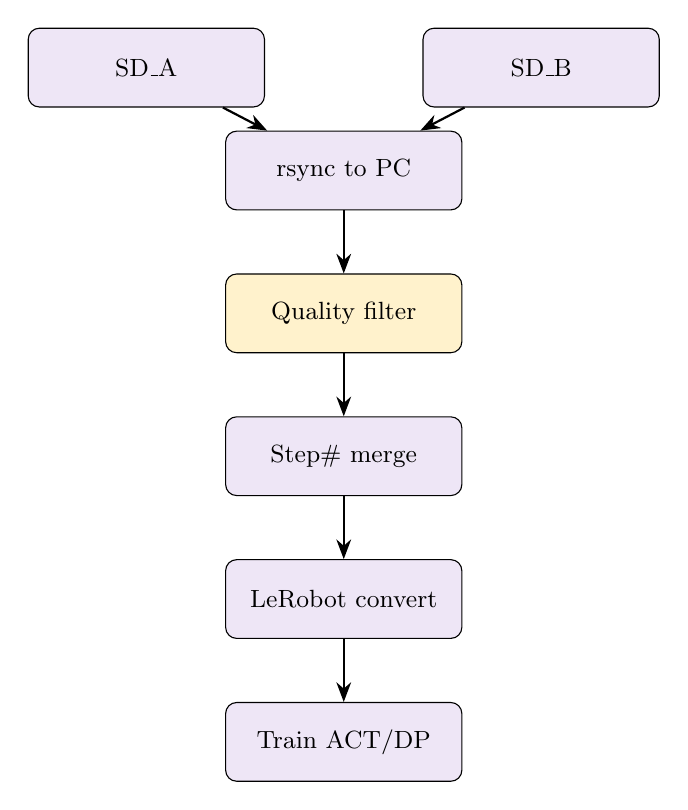
\begin{tikzpicture}[
  node distance=8mm,
  every node/.style={draw, rounded corners=4pt, minimum width=30mm, minimum height=10mm, align=center, font=\small},
  arr/.style={-{Stealth[length=2.5mm]}, thick},
]
  \node[fill=nodepurple!60!white] (l) {SD\_A};
  \node[fill=nodepurple!60!white, right=20mm of l] (r) {SD\_B};
  \node[fill=nodepurple!60!white, below=of $(l)!0.5!(r)$] (xfer) {rsync to PC};
  \node[fill=nodeyellow, below=of xfer] (filter) {Quality filter};
  \node[fill=nodepurple!60!white, below=of filter] (merge) {Step\# merge};
  \node[fill=nodepurple!60!white, below=of merge] (conv) {LeRobot convert};
  \node[fill=nodepurple!60!white, below=of conv] (train) {Train ACT/DP};

  \draw[arr] (l) -- (xfer);
  \draw[arr] (r) -- (xfer);
  \draw[arr] (xfer) -- (filter);
  \draw[arr] (filter) -- (merge);
  \draw[arr] (merge) -- (conv);
  \draw[arr] (conv) -- (train);
\end{tikzpicture}
\caption{Post-collection pipeline with quality filtering. Episodes with confidence $< 2$ are automatically discarded.}
\label{fig:pipeline}
\end{figure}


% ════════════════════════════════════════════════════════════
% 8. Performance Analysis
% ════════════════════════════════════════════════════════════
\section{Performance Analysis}

% ─────────────────────────────────────────────────
% 8.1 Latency Breakdown
% ─────────────────────────────────────────────────
\subsection{Latency Breakdown}

\begin{table}[htbp]
\centering
\caption{Latency breakdown for a single NRF round trip with 32-byte payload and ACK payload.}
\begin{tabular}{l r r l}
\toprule
\textbf{Phase} & \textbf{Duration} & \textbf{Cumulative} & \textbf{Notes} \\
\midrule
SPI TX (32B at 8\,MHz) & ${\sim}$26\,$\mu$s & 26\,$\mu$s & 32 bytes $\times$ 8 bits / 8\,MHz \\
PLL lock & 130\,$\mu$s & 156\,$\mu$s & Crystal stabilization \\
On-air TX (2\,Mbps) & 164.5\,$\mu$s & 320.5\,$\mu$s & Full packet / 2\,Mbps \\
Receiver processing & ${\sim}$10\,$\mu$s & 330.5\,$\mu$s & Address match + CRC \\
ACK TX (2\,Mbps, 32B) & 164.5\,$\mu$s & 495\,$\mu$s & ACK with payload \\
SPI RX (ACK payload) & ${\sim}$26\,$\mu$s & 521\,$\mu$s & Read ACK from FIFO \\
Software overhead & ${\sim}$36\,$\mu$s & 557\,$\mu$s & Timestamp, pack/unpack \\
\midrule
\textbf{Theoretical RTT} & & \textbf{${\sim}$557\,$\mu$s} & \\
\textbf{Measured RTT} & & \textbf{${\sim}$800\,$\mu$s} & Linux scheduling adds ${\sim}$243\,$\mu$s \\
\bottomrule
\end{tabular}
\label{tab:latency}
\end{table}

% ─────────────────────────────────────────────────
% 8.2 Sync Error Comparison
% ─────────────────────────────────────────────────
\subsection{Sync Error Comparison}

\begin{table}[htbp]
\centering
\caption{Sync error comparison: WiFi UDP vs NRF24L01+.}
\begin{tabular}{l c c c}
\toprule
\textbf{Metric} & \textbf{WiFi UDP} & \textbf{NRF24L01+} & \textbf{Improvement} \\
\midrule
Mean RTT & ${\sim}$2.0\,ms & ${\sim}$0.8\,ms & 2.5$\times$ \\
RTT std dev & ${\sim}$0.5\,ms & ${\sim}$0.15\,ms & 3.3$\times$ \\
Sync error (10-round) & ${\sim}$0.5\,ms & ${\sim}$0.2\,ms & 2.5$\times$ \\
Max sync error & ${\sim}$1.5\,ms & ${\sim}$0.4\,ms & 3.7$\times$ \\
Drift after 300 steps & ${\sim}$0.2\,ms & ${\sim}$0.2\,ms & Same (crystal) \\
Error bound & Constant & Constant & Both bounded \\
\bottomrule
\end{tabular}
\label{tab:sync-comparison}
\end{table}

% ─────────────────────────────────────────────────
% 8.3 Step Timing at 30Hz
% ─────────────────────────────────────────────────
\subsection{Step Timing at 30\,Hz}

\begin{table}[htbp]
\centering
\caption{Single-step timing breakdown at 30\,Hz (33.3\,ms frame period). NRF duty cycle ${\sim}$2.4\%.}
\setlength{\tabcolsep}{4pt}
\begin{tabular}{l c c c c c}
\toprule
 & 0--0.8\,ms & 0.8--1\,ms & 1--5\,ms & 5--32\,ms & 32--33.3\,ms \\
\midrule
\textbf{NRF radio} & \cellcolor{nodered}TX+ACK & \cellcolor{nodered}proc & & & \\
\textbf{Sensors} & & \cellcolor{nodeblue}latch & \cellcolor{nodeblue}T265+RGB & & \\
\textbf{Disk} & & & & \cellcolor{nodegreen}write & \\
\textbf{Idle} & & & & & \cellcolor{black!8}sleep \\
\midrule
\textbf{Duty} & \multicolumn{2}{c}{\cellcolor{nodeyellow}${\sim}$3\%} & \cellcolor{nodeyellow}${\sim}$12\% & \cellcolor{nodeyellow}${\sim}$80\% & \cellcolor{nodeyellow}${\sim}$5\% \\
\bottomrule
\end{tabular}
\label{tab:step-timing}
\end{table}

% ─────────────────────────────────────────────────
% 8.4 Power Consumption
% ─────────────────────────────────────────────────
\subsection{Power Consumption}

\begin{table}[htbp]
\centering
\caption{Power comparison. NRF24L01+ consumes ${\sim}$3000$\times$ less power than WiFi.}
\begin{tabular}{l c c l}
\toprule
\textbf{State} & \textbf{NRF24L01+} & \textbf{WiFi (BCM43455)} & \textbf{Notes} \\
\midrule
TX active & 11.3\,mA & ${\sim}$300\,mA & NRF at 0\,dBm; WiFi at ${\sim}$20\,dBm \\
RX active & 13.5\,mA & ${\sim}$100\,mA & Listening for packets \\
Standby-I & 26\,$\mu$A & N/A & NRF between transactions \\
Power down & 900\,nA & N/A & Not used during recording \\
\midrule
\textbf{Average at 30\,Hz} & \textbf{${\sim}$50\,$\mu$A} & \textbf{${\sim}$150\,mA} & NRF: 2.4\% duty cycle \\
\textbf{Daily energy (24h)} & \textbf{${\sim}$4\,mWh} & \textbf{${\sim}$12\,Wh} & NRF: negligible \\
\bottomrule
\end{tabular}
\label{tab:power}
\end{table}

\begin{infobox}[Measured vs Theoretical]
The ${\sim}$243\,$\mu$s gap between theoretical (557\,$\mu$s) and measured (800\,$\mu$s) RTT is caused by Linux scheduling latency. The RPi 4B runs a non-realtime kernel; context switches add 50--200\,$\mu$s jitter. This jitter is \emph{symmetric} (affects both peers equally on average), so it cancels in the offset calculation. The offset estimate remains accurate to within $\pm$0.2\,ms after multi-round averaging.
\end{infobox}


% ════════════════════════════════════════════════════════════
% 9. TODO
% ════════════════════════════════════════════════════════════
\section{TODO}

This section lists tasks required to build and validate the complete bimanual data collection system.

\subsection{Procurement and Unit Tests}

\textbf{Goal:} Confirm every component works individually.

\begin{itemize}[label=$\square$]
  \item Acquire 2 T265 cameras (eBay / AliExpress). Verify firmware version 0.2.0.951.
  \item Flash Ubuntu 22.04 Server 64-bit on both RPi 4Bs.
  \item Build librealsense v2.53.1 from source with FORCE\_RSUSB\_BACKEND and Python bindings.
  \item Add T265 USB autosuspend udev rule.
  \item Enable GPIO UART on /dev/ttyAMA0. Verify STS3215 position read at 100\,Hz.
  \item Enable SPI0 for NRF24L01+. Verify radio link with pyrf24 ping-pong test.
  \item Test USB RGB camera (wowrobo) at 1080p@30fps via OpenCV.
\end{itemize}

\subsection{Single Gripper Recorder}

\textbf{Goal:} Record one gripper's data to SD at 30\,Hz.

\begin{itemize}[label=$\square$]
  \item Implement T265 callback: buffer pose at 200\,Hz, capture fisheye at 30\,Hz.
  \item Implement USB RGB capture thread at 30\,Hz.
  \item Implement STS3215 UART polling thread at 100\,Hz.
  \item Build 5-way synchronizer: on NRF trigger, match nearest pose ($\pm$2.5\,ms), fisheye ($\pm$16.7\,ms), RGB ($\pm$16.7\,ms), and gripper ($\pm$5\,ms).
  \item Implement episode recorder with GPIO button and LED indicator.
  \item Save episodes to SD card. Verify sustained 30\,Hz write.
  \item Build playback visualizer.
\end{itemize}

\subsection{NRF Bimanual Synchronization}

\textbf{Goal:} Two grippers capture in lockstep via NRF24L01+.

\begin{itemize}[label=$\square$]
  \item Wire NRF24L01+ modules to both RPis with bypass capacitors.
  \item Implement 32-byte NRF packet format.
  \item Implement time synchronization phase with ACK payload (10 rounds, outlier rejection).
  \item Implement alternating trigger loop: even steps by PTX, ACK payload from PRX.
  \item Implement packet-loss detection with empty frame insertion.
  \item Add periodic re-sync every 300 steps.
  \item Stress test: 10-minute continuous run. Verify A/B step counts match exactly.
  \item Validate: average RTT $<$ 1\,ms; zero step misalignment after 10 minutes.
\end{itemize}

\subsection{Hardware Integration}

\textbf{Goal:} Two complete wireless gripper units with NRF and dual cameras.

\begin{itemize}[label=$\square$]
  \item Design 3D housing: T265 mount, RPi slot, NRF antenna clearance, USB RGB mount, LiPo bay, STS3215 mechanism, ergonomic handle.
  \item Print (PLA frame + TPU fingertips), assemble, and wire both units.
  \item Gripper calibration: STS3215 encoder count $\to$ mm aperture.
  \item Battery endurance test: confirm 45+ min per charge.
\end{itemize}

\subsection{Pilot Data Collection}

\textbf{Goal:} 50+ bimanual demonstration episodes.

\begin{itemize}[label=$\square$]
  \item Collect tabletop pick-and-place tasks.
  \item Auto-quality filter: discard episodes where confidence drops below 2.
  \item Transfer via rsync. Run merge script matching step numbers.
  \item Verify merged dataset integrity.
\end{itemize}

\subsection{Policy Training and Deployment}

\textbf{Goal:} Close the loop from data to autonomous execution.

\begin{itemize}[label=$\square$]
  \item Convert merged episodes to LeRobot dataset format.
  \item Train Diffusion Policy or ACT on fisheye + RGB observation + pose state.
  \item Mount T265 + gripper on SO-101 follower arm wrist.
  \item Evaluate autonomous bimanual task execution.
\end{itemize}


% ════════════════════════════════════════════════════════════
% 10. Risk Assessment
% ════════════════════════════════════════════════════════════
\section{Risk Assessment}

\begin{table}[htbp]
\centering
\caption{Key risks and mitigation strategies (updated for NRF24L01+).}
\begin{tabular}{l c p{7cm}}
\toprule
\textbf{Risk} & \textbf{Level} & \textbf{Mitigation} \\
\midrule
T265 unavailable (discontinued) & Med & Buy 2+ units now; fallback: OAK-D Lite + DepthAI VIO \\
librealsense ARM64 build failure & Med & v2.53.1 + FORCE\_RSUSB\_BACKEND verified on RPi4 \\
Mono fisheye hurts policy & Low & USB RGB camera added as secondary observation \\
NRF24L01+ SPI failure & Low & Bypass caps + STATUS register check; fallback to WiFi UDP \\
NRF range insufficient & Low & Basic module covers 10\,m; PA+LNA variant for longer range \\
2.4\,GHz interference & Low & Channel 108 above WiFi; auto-retry handles transient loss \\
RPi thermal throttle & Low & Heatsink + fan; 15-min sessions with battery swap \\
STS3215 UART unstable & Low & 74HC126 buffer IC or USB-serial adapter fallback \\
\bottomrule
\end{tabular}
\label{tab:risks}
\end{table}


% ════════════════════════════════════════════════════════════
% 11. Conclusion
% ════════════════════════════════════════════════════════════
\section{Conclusion}

This report presented a low-cost wireless bimanual data collection system designed for imitation learning. Key contributions include:

\begin{enumerate}
  \item \textbf{Fully wireless architecture:} Each gripper unit operates independently with onboard compute and battery, eliminating tethering constraints during data collection.

  \item \textbf{NRF24L01+ synchronization:} Enhanced ShockBurst with hardware ACK payload achieves ${\sim}$0.8\,ms RTT and ${\sim}$0.2\,ms sync error, a 2.5$\times$ improvement over WiFi UDP.

  \item \textbf{Dual-camera integration:} T265 fisheye for VIO and wide-angle observation, plus USB RGB for close-range color observation, providing rich multi-modal data for policy learning.

  \item \textbf{Step-based alignment:} Absolute step numbers enable trivial post-collection merging without complex timestamp alignment algorithms.

  \item \textbf{Cost efficiency:} The complete bimanual system costs approximately \$676, significantly less than alternatives requiring external tracking infrastructure.

  \item \textbf{Robust error handling:} Three-tier failure recovery (hardware retry, software timeout, RESYNC) ensures continuous operation despite transient radio issues.
\end{enumerate}

Future work includes integrating the system with the SO-101 robot arm for closed-loop policy evaluation and exploring multi-gripper configurations beyond bimanual setups.


% ════════════════════════════════════════════════════════════
% 12. References
% ════════════════════════════════════════════════════════════
\section{References}

\subsection{QR Code Quick Links}

\begin{figure}[htbp]
\centering
\begin{tabular}{ccc}
\qrcode[height=2.5cm]{https://www.nordicsemi.com/Products/nRF24-series} &
\qrcode[height=2.5cm]{https://nrf24.github.io/RF24/} &
\qrcode[height=2.5cm]{https://pinout.xyz/} \\
NRF24L01+ Datasheet & pyRF24 Documentation & RPi GPIO Pinout \\[12pt]
\qrcode[height=2.5cm]{https://www.intelrealsense.com/tracking-camera-t265/} &
\qrcode[height=2.5cm]{https://github.com/huggingface/lerobot} &
\qrcode[height=2.5cm]{https://www.youtube.com/watch?v=vJqyUTTbo6I} \\
Intel T265 Camera & LeRobot Framework & UMI Gripper Tutorial \\
\end{tabular}
\caption{QR codes for key references.}
\label{fig:qrcodes}
\end{figure}

\subsection{Reference URLs}

\begin{table}[htbp]
\centering
\begin{tabular}{l l}
\toprule
\textbf{Resource} & \textbf{URL} \\
\midrule
NRF24L01+ Datasheet & nordicsemi.com/Products/nRF24-series \\
pyRF24 Library & nrf24.github.io/RF24/ \\
RPi GPIO Pinout & pinout.xyz \\
Intel RealSense T265 & intelrealsense.com/tracking-camera-t265/ \\
wowrobo USB Camera & wowrobo.com (SO-ARM100/101 compatible) \\
LeRobot Framework & github.com/huggingface/lerobot \\
UMI Gripper (Stanford) & umi-gripper.github.io \\
Diffusion Policy & github.com/real-stanford/diffusion\_policy \\
ACT (Aloha) & github.com/tonyzhaozh/act \\
\bottomrule
\end{tabular}
\caption{Complete reference URL list.}
\label{tab:urls}
\end{table}


\end{document}
